\section{Analysis}
\label{analysis}
%Our analysis of the paper and algorithm goes here
%From the course's intended learning outcomes (ILO):
%"Find, extract and explain results in the algorithms research literature relevant to a given problem"
%"Theoretically analyze the performance of a given algorithmic solution"

\subsection{Building the sketch}
The sketch is a compressed representation of a point set \texttt{X}. The points of \texttt{X} have \texttt{d} dimensions and are in \textit{euclidean} space. Each coordinate of a point is represented by \texttt{B} bits implying a point is represented by \textit{dB} bits. \qs{} will take as input the point set \texttt{X} and two additional parameters \texttt{L} and $\Lambda$. These two parameters are used to specify the compression of the point set where \texttt{L} is the depth of the \qt{} and $\Lambda$ is the amount of nodes from the \qt{} which can be removed. 
%TODO: PRÆCISÉR parametre
There are three steps for building the sketch: randomly shifted grid, \qt{} construction and pruning. These steps will be explained briefly and there will be given an example of how a sketch is built on a small example.
\\
\\
The first step is randomly shifted grid. Here there is constructed a hypercube \texttt{H} which contains all points of the given point set \texttt{X}. \texttt{H} will then be set up to be centered around a point of \texttt{X}. Then choose a random value $\sigma$ for each dimension of the hypercube. For each dimension \texttt{j} of \texttt{H} will be shifted with $\sigma_j$.
\\
\\
The next step is creating the \qt{}. A \textit{2d-ary} \qt{} is created by starting at the root of \texttt{H}. There is then only added the children which contain a point from \texttt{X}, thus child nodes that do not contain a point from \texttt{X} are ignored. Each edge to a child node is labeled with a \textit{d} long bit string that has been split on. This step is then done recursively until the level \texttt{L} is reached. An example of a constructed \qt{} is given in figure \ref{fig:quadtree}.

%TODO: SÆT STØRRELSEN OP MAND på font størelsen!!!
\begin{figure}
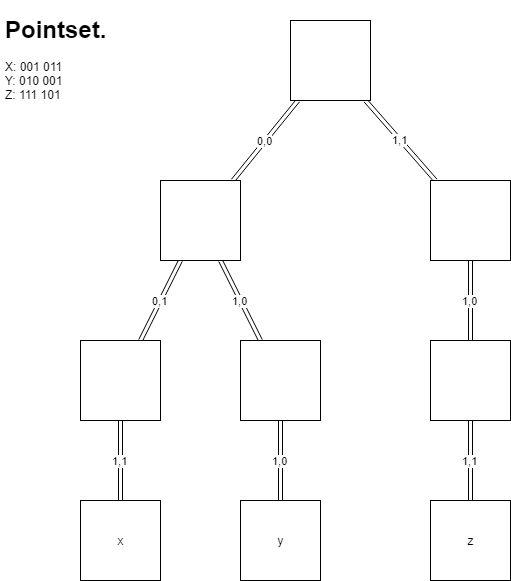
\includegraphics[width=0.5\textwidth]{figures/quadtree}
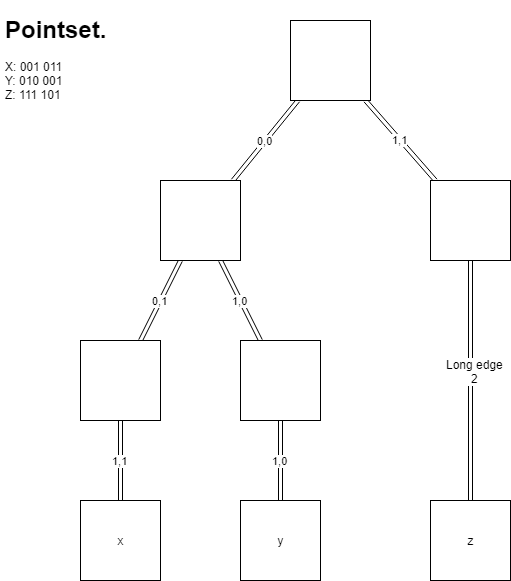
\includegraphics[width=0.5\textwidth]{figures/prunnedquadtree}
\caption{On the left there is shown the \qt{} after construction with $L=4$. On the right the \qt{} has been pruned with a $\Lambda = 1$}
\label{fig:quadtree}
\end{figure}

After construction of the \qt{} the tree is pruned. There are found downward paths $n_0,...,n_k$ where nodes $n_1,...,n_{k-1}$ all have a degree 1. If \ensuremath{\texttt{k} > \Lambda+1} then there are removed nodes $n_{\Lambda+1},...,n_{k-1}$ from the \qt{}. Instead node $n_{\Lambda}$ is connected directly to $n_{k}$ with an edge. This edge is called a long edge and is labeled with the length of the path it replaces. This is given an example of the tree after a pruning in figure \ref{fig:quadtree}.


From this the sketch can be built. There is used the "Eulerian Tour Technique"\footnote{See e.g., \url{https://en.wikipedia.org/wiki/Euler\_tour\_technique}}.
It starts at the root an searches down to the leftmost leaf. It will then back track up to its parents until it finds an new leaf it can traverse down to. When an edge is explored downwards there is stored a 0 and the label of the edge either a bit string or the length of an long edge. Also for each downward movement there is stored a bit specifying if the given edge is a long or short edge. If an upwards edge is explored then a 1 is stored. Furthermore, there is stored for each point an index for the child node which contains it.

\subsection{Why randomly shift hypercube?}
Randomly shifting a hypercube in each dimension is necessary for the \qs{} implementation to maintain guarantees on arbitrary datasets. We hope to obtain a cube in which data points near each other are shifted into the same leaves in the \qt{}. The shifting can have varying practical effects given the randomness of the shifting.
\\
\\
If the dataset is of a known format, randomly shifting it in each dimension could turn out to be less effective than taking a more specific approach. An example could be a dataset in which all the points are very close to each other. A large amount of the points might end up in the same leaves and as such defeat the purpose of using the \qt{} to begin with. Randomly shifting over these points will not be of any significant gain to the problem at hand. One approach could be to spread out the dataset in the sense of scaling the points given some constant to increase the distance between them and hereby obtain a \qt{} of a better quality. The original relative distance is preserved by remembering the scaling constant.

\subsection{Theorems}

\subsubsection{Aspect ratio}
The aspect ratio is defined as the ratio between the largest and smallest distance between points in the dataset\cite{wagner17}. The aspect ratio is denoted as $\Phi$:
\\
\\
$$ \Phi = \frac{max_{1<i<j<n} || x_i - x_j || }{min_{1<i<j<n} || x_i - x_j || } $$
\\
\\
The aspect ratio can be used to gain insight about the distribution of data points in euclidean space. When $\Phi$ approaches 1 then points are clustered close together. When $\Phi$ grows then the points are more spread out in the point space but will not describe how the points are spread. There could be an outlier which gives a big $\Phi$. If some point set p is distributed in a euclidean space, the quad sketch will need more bits to precisely describe the position of points in p. Hence $\Phi$ has an impact on how the parameters $\Lambda$ and $\L$ should be set to dictate the guarantees of the sketch.

\subsubsection{Theorems}
The paper introduces three theorems, where \tm{1} is the main theorem covering the basic variant of \qs{}. \tm{2} covers an advanced variant, and \tm{3} is the full version. The former makes guarantees for a \qs{} variant, where “for each point, the distances from that point to all other points are preserved up to a factor of 1+- $\epsilon$ with a constant probability”, whereas the latter “makes it possible to approximately preserve the distances between all pairs of points”. It seems like \tm{1} thus allows us to find distances between one single point and to all other points, but not the other way around, whereas with \tm{2} we can find the distance both from node 1 to node 2 and 3, but also from node 2 to node 3. This comes with a trade off, as with \tm{1} you are able to recover any points by decompressing the sketch, which is infeasible with \tm{2}, where \qs{} is recursively applied.

%(TODO: Then what is theorem 3?)